\documentclass[11.5pt, paper=a4]{article}

\usepackage[utf8]{inputenc}
\usepackage[english]{babel}
\usepackage[T1]{fontenc}

\usepackage{amsmath, amssymb, amscd, amsthm, amsfonts, mathtools}
\usepackage[left=2cm, right=2cm, top=1.5cm]{geometry}

\usepackage{graphicx}
\usepackage{hyperref}
\usepackage{physics}
\usepackage{tikz}
\usepackage{url}
\usepackage[square,numbers]{natbib} \usepackage{tabularx}

\usepackage{braket}
\usepackage{thmtools}
\usepackage{float}

%%% Theorem Style
\theoremstyle{definition}
\newtheorem{theorem}{Theorem}[section]
\newtheorem{definition}[theorem]{Definition}
\newtheorem{lemma}[theorem]{Lemma}
\newtheorem{conjecture}[theorem]{Conjecture}
\newtheorem{corollary}[theorem]{Corollary}

\numberwithin{theorem}{section}

%% Autoref prefixes
\renewcommand{\sectionautorefname}{Section}
\renewcommand{\subsectionautorefname}{Section}
\renewcommand{\subsubsectionautorefname}{Section}
\renewcommand{\figureautorefname}{Figure}
\def\theoremautorefname{Theorem}
\def\lemmaautorefname{Lemma}
\def\definitionautorefname{Definition}
\def\conjectureautorefname{Conjecture}
\def\algorithmautorefname{Algorithm}

%% Writing algorithms

\usepackage{algorithm} % captioning
\usepackage{algpseudocode}

% \def\NoNumber#1{{\def\alglinenumber##1{}\State #1}\addtocounter{ALG@line}{-1}}



\title{Quantum Algorithms, Spring 2022: Lecture 2 Scribe}

\author{Pratishtha Abrol, Kushagra Garg}

\date{January 7, 2022}

\begin{document}

\maketitle
\section{Recap}
We had introduced the course in the first lecture and provided the physical, computational and philosophical motivation for the Quantum computing. Starting with Maxwell's daemon and Landauer's principle we asserted that information is physical. Then we discussed the historical developments, the key events and current and future outlook for the field of Quantum Computing.
In this lecture, we will learn some of the basic concepts of quantum computing and will develop the mathematical tools and framework required.

\section{Quantum Mechanics in a Nutshell}
Quantum Mechanics is the mathematical modelling of the actual physical world which governs subatomic particles. Since quantum systems are very fragile and tend to lose their "quantum-ness" on interaction with the environment, quantum mechanics is actually a description of perfectly isolates quantum systems, that is, quantum systems that are insulated from noise.

When we talk about classical physics, of a particle with an initial velocity and particular initial local coordinates, we can describe this particle with, say a vector. Such a classical system is governed by equations of motion, which can describe the trajectory of the motion of the particle and it's properties (location/speed) at any time \textit{t}.
As opposed to a classical state, a quantum state is a linear combination (\textit{superposition}) of classical states, which can be written as a vector of complex amplitudes, to which we either apply a unitary operation (\textit{to evolve the system to a new quantum state}) or perform a measurement (\textit{to observe an outcome}).

\section{Qubit}
The qubit is the quantum equivalent of a bit. It is the fundamental unit of quantum computation and information, just as bit is for classical information.
A bit, is classically in one of the two states: "0" or "1". In contrast, a qubit can be in $\ket{0}$ or $\ket{1}$ or in any superposition (linear combination) of the two.
\begin{equation} \label{eq:1}
    \ket{\psi} = \alpha \ket{0} + \beta \ket{1}; \alpha, \beta \in C
\end{equation}
where, $\ket{\psi}$ is unit vector in 2-D complex inner-product space, i.e. the Hilbert Space, and, \\
\begin{center}
$\ket{0} =
\begin{pmatrix}
1 \\
0
\end{pmatrix} $ and $\ket{1} =
\begin{pmatrix}
0 \\
1
\end{pmatrix}    $
\end{center}
which are computational basis states that span the 2 dimensional vector space/ form an orthonormal basis for this vector space.

On measurement we get either the result 0, with probability  $\norm{\alpha^2}$ , or 1, with probability $\norm{\beta^2}$. Naturally, it implies
\begin{equation}
\braket{{\psi}|{\psi}}= \norm{\alpha^2}+ \norm{\beta^2} = 1
\end{equation}
So, qubit is a unit vector. Using this, we can write  [\ref{eq:1}] as
\begin{equation}
    \ket{\psi} = e^{i\gamma}\big(\cos{\frac{\theta}{2}}\ket{0} + e^{i\phi} \sin{\frac{\theta}{2}}\ket{0}\big)
\end{equation}
\begin{figure}[h]
\centering
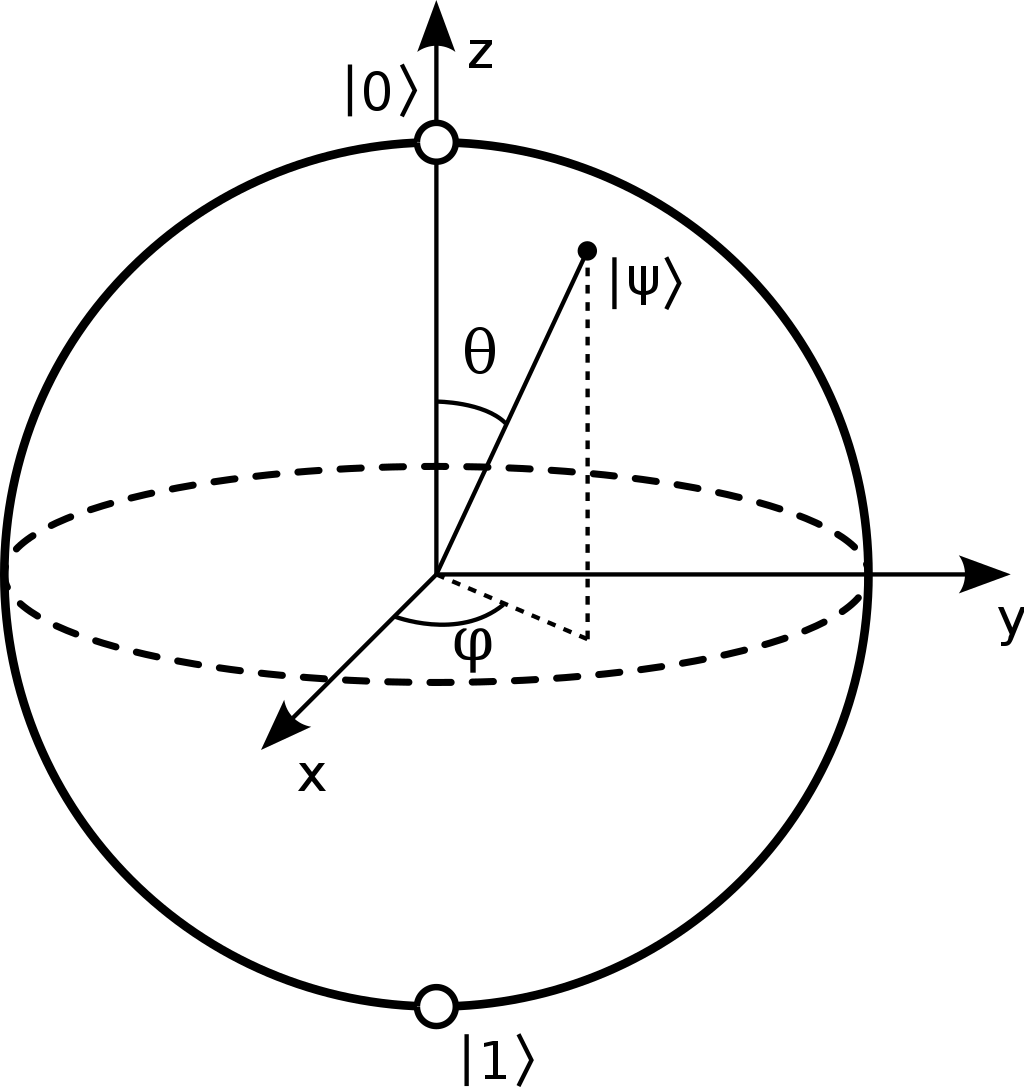
\includegraphics[width=0.4\linewidth]{bloch_sphere.png}
\caption{Bloch sphere. \cite{bloch_sphere}}
\label{fig:Bloch sphere}
\end{figure}

where $\theta$, $\phi$ and $\gamma$ are real. The factor of $e^{i\gamma}$, called global phase, has no observable effects and can be ignored. The qubit can be represented as a point on a three-dimensional sphere called as \textit{Bloch sphere} fig.\ref{fig:Bloch sphere}.

Qubits can be manipulated in a way that their states interact/interfere to leads to a quantum state, which when measures, leads to the outcome we desire.

A qubit represents a physical entity. Some of the ways it can be manifested are Polarization of light, Spin of an electron, etc \cite{physical_qubits}.


\section{Multiple Qubits}
\begin{itemize}
    \item Pairs of qubits, the 4 possible computational basis states include: $\ket{00}, \ket{01}, \ket{10}, \ket{11}$ each of which is a tensor product shorthand (i.e. $\ket{01} = \ket{0} \otimes \ket{1} =
    \begin{pmatrix}
    0 \\
    1 \\
    0 \\
    0
    \end{pmatrix}) $
    \item Naturally, an $n$ dimensional qubit state "lives in" a $2^n$ dimensional Hilbert space.
\end{itemize}


\section{Postulates of Quantum Mechanics}
\textbf{Postulate 1 (P1):} Any physical system has, associated with it, a complex vector space with inner product (Hilbert Space), known as the state space of the system. The state of an isolated physical system is represented by $\ket{\psi}$ denoting a unit vector in the system's state space.
\begin{itemize}
    \item A system has a state space $\mathcal{H}$ of dimension $d$ and is in a state $\ket{\psi} \in \mathcal{H}$.
    \begin{equation*}
        \ket{\psi} = a\ket{0} + b\ket{1}, \ket{\psi} \in C^2
    \end{equation*}
    \item Any two states, say $\ket{\psi_i}$ and $\ket{\psi_j}$ are orthonormal if $\braket{\psi_j|\psi_j} = \delta_{ij}$.
    \item $\ket{\psi} = e^{i\phi} \ket{\psi}$
    \item Any linear combination $\sum_i \alpha_i \ket{\psi_i}$ is a superposition of states $\ket{\psi_i}$ with amplitudes $\alpha_i$.
\end{itemize}


\textbf{Postulate 2 (P2):} The state space of a composite physical system is a tensor product of the component physical systems. Suppose you have a system $S_i$ of state space $\mathcal{H}_i$, where $i \in \{1,2,...,n\}$, then the state space of the joint system is $\mathcal{H_1} \otimes \mathcal{H_2} \otimes ... \otimes \mathcal{H_n}$, and would belong to $\mathcal{H}$.
\begin{itemize}
    \item Say we have an $n$ qubit system, the state space dimension would be: $C^2 \otimes C^2 \otimes ... \otimes C^2$ ($n$ times) = $C^{2^n}$.
\end{itemize}

\section{In Class Exercise}
Suppose you have $\ket{\psi} = \sum_{i=1}^n a_i \ket{i}$, such that $\sum_{i=1}^n \norm{a_i}^2 = 1$ and $\ket{\phi} = \sum_{j=1}^m b_i \ket{j}$, such that $\sum_{j=1}^m \norm{b_i}^2 = 1$. What is $\ket{\gamma} = \ket{\psi}\ket{\phi}$?
\\
\\
\textbf{Answer.} Obviously, $dim(\gamma) = mn$.
\begin{equation*}
    \ket{\gamma} = \sum_{i=1,j=1}^{i=n, j=m} a_i b_j \ket{i} \ket{j}
\end{equation*}
\nocite{nielsen00}
\nocite{preskill}
\bibliographystyle{plainnat}
\bibliography{references}


\end{document}

